\documentclass[]{article}
\usepackage{lmodern}
\usepackage{amssymb,amsmath}
\usepackage{ifxetex,ifluatex}
\usepackage{fixltx2e} % provides \textsubscript
\ifnum 0\ifxetex 1\fi\ifluatex 1\fi=0 % if pdftex
  \usepackage[T1]{fontenc}
  \usepackage[utf8]{inputenc}
\else % if luatex or xelatex
  \ifxetex
    \usepackage{mathspec}
  \else
    \usepackage{fontspec}
  \fi
  \defaultfontfeatures{Ligatures=TeX,Scale=MatchLowercase}
\fi
% use upquote if available, for straight quotes in verbatim environments
\IfFileExists{upquote.sty}{\usepackage{upquote}}{}
% use microtype if available
\IfFileExists{microtype.sty}{%
\usepackage{microtype}
\UseMicrotypeSet[protrusion]{basicmath} % disable protrusion for tt fonts
}{}
\usepackage[margin=1in]{geometry}
\usepackage{hyperref}
\hypersetup{unicode=true,
            pdftitle={Agenda},
            pdfauthor={Yohan Min},
            pdfborder={0 0 0},
            breaklinks=true}
\urlstyle{same}  % don't use monospace font for urls
\usepackage{graphicx,grffile}
\makeatletter
\def\maxwidth{\ifdim\Gin@nat@width>\linewidth\linewidth\else\Gin@nat@width\fi}
\def\maxheight{\ifdim\Gin@nat@height>\textheight\textheight\else\Gin@nat@height\fi}
\makeatother
% Scale images if necessary, so that they will not overflow the page
% margins by default, and it is still possible to overwrite the defaults
% using explicit options in \includegraphics[width, height, ...]{}
\setkeys{Gin}{width=\maxwidth,height=\maxheight,keepaspectratio}
\IfFileExists{parskip.sty}{%
\usepackage{parskip}
}{% else
\setlength{\parindent}{0pt}
\setlength{\parskip}{6pt plus 2pt minus 1pt}
}
\setlength{\emergencystretch}{3em}  % prevent overfull lines
\providecommand{\tightlist}{%
  \setlength{\itemsep}{0pt}\setlength{\parskip}{0pt}}
\setcounter{secnumdepth}{0}
% Redefines (sub)paragraphs to behave more like sections
\ifx\paragraph\undefined\else
\let\oldparagraph\paragraph
\renewcommand{\paragraph}[1]{\oldparagraph{#1}\mbox{}}
\fi
\ifx\subparagraph\undefined\else
\let\oldsubparagraph\subparagraph
\renewcommand{\subparagraph}[1]{\oldsubparagraph{#1}\mbox{}}
\fi

%%% Use protect on footnotes to avoid problems with footnotes in titles
\let\rmarkdownfootnote\footnote%
\def\footnote{\protect\rmarkdownfootnote}

%%% Change title format to be more compact
\usepackage{titling}

% Create subtitle command for use in maketitle
\newcommand{\subtitle}[1]{
  \posttitle{
    \begin{center}\large#1\end{center}
    }
}

\setlength{\droptitle}{-2em}

  \title{Agenda}
    \pretitle{\vspace{\droptitle}\centering\huge}
  \posttitle{\par}
    \author{Yohan Min}
    \preauthor{\centering\large\emph}
  \postauthor{\par}
      \predate{\centering\large\emph}
  \postdate{\par}
    \date{November 26, 2018}


\begin{document}
\maketitle

{
\setcounter{tocdepth}{2}
\tableofcontents
}
\subsection{Energy code}\label{energy-code}

\subsubsection{Title 24 vs.~IECC}\label{title-24-vs.iecc}

연방정부 기준인 IECC 를 적어도 만족시키는 주정부 energy 기준이 있어야
하는데, CA 의 경우 2016 Building Energy Efficiency Standards Title 24,
Part 6 이 2015 IECC 를 넘어서는 결과를 보여주고 있다.

\subsubsection{2018 IECC}\label{iecc}

가장 최근 버전으로 - APPENDIX RA SOLAR-READY PROVISIONS---DETACHED ONE-
AND TWOFAMILY DWELLINGS, MULTIPLE SINGLE-FAMILY DWELLINGS (TOWNHOUSES) -
solar ready 에 대한 조건이 있다.

\subsubsection{2019 Residential Compliance
Manual}\label{residential-compliance-manual}

CA 에서 나온 것으로, PV 설치를 강제하고 있고, 예외에 한에서 역시 solar
ready 를 강제하고 있다. Seattle 이 경우 2017 residential code 가 해당.
Residential 의 경우 solar ready 는 residential code 에 있는데,
commercial 의 경우 solar ready 는 building code 가 아닌 energy code 에
있다. 참고로, single family 와 low rise multifamily 는 residential code
(특별 building code 로 보면 될 듯), 그 외는 building code. 그리고 solar
를 직접 설치 했을 때는 NEC 의 electrical code 와 관계한 electrical
permit 을 받아야 한다.

\begin{quote}
The California Energy Code, part 6 of the California Building Standards
Code which is title 24 of the California Code of Regulations, also
titled The Energy Efficiency Standards for Residential and
Nonresidential Buildings, were created by the California Building
Standards Commission in 1978 in response to a legislative mandate to
reduce California's energy consumption. The standards are updated
periodically by the California Energy Commission to allow consideration
and possible incorporation of new energy efficiency technologies and
methods. The California Energy Code (CEC) contains energy conservation
standards applicable to most residential and nonresidential buildings
throughout California, including schools. - solar ready, residential
compliance manual.
\end{quote}

\begin{quote}
There are 3 different kinds of building codes: private sector, federal
sector, and international. The private sector codes are associated with
state and local jurisdiction. States and local jurisdictions have
different energy codes that they follow based on climate, geography, and
many other contributing factors. The two primary baseline codes for the
private sector are the International Energy Conservation Code (IECC),
and the ANSI/ASHRAE/IESNA Standard 90.1 energy standard for Buildings
Except Low-Rise Residential Buildings (ASHRAE 90.1).{[}4{]} States and
local governments adopt and enforce these energy codes. The standards
are published by national organizations such as ASHRAE. The
International Code Council (ICC) develops the codes and standards used
to construct residential and commercial buildings, including homes and
schools.{[}5{]} Within the ICC is the IECC which is a subset of the ICC.
The IECC is a model energy code, but it is written in mandatory,
enforceable language, so that state and local jurisdictions can easily
adopt the model as their energy code.{[}6{]} The IECC references several
ASHRAE Standards, in particular the ASHRAE 90.1 for commercial building
construction.
\end{quote}

\subsection{OSHA}\label{osha}

\begin{itemize}
\item
  Roof slope: OSHA defines a low-slope roof as a roof having a slope of
  less than or equal to 4 inches of vertical rise for every 12 inches
  horizontal length (4:12) (1926.500(b)---definitions). This is
  important because the OSHA definition is used as a basis for
  implementing low-slope fall-protection measures, such as warningline
  systems and safety monitors.
\item
  Ladder: angle 75 degree, one-quarter the working length of the ladder
  (a 1:4 ratio) (29 CFR 1926.1053(b)(5)(i)). 3 rungs (1 ft apart) above
  the roof, The side rails of the ladder generally must extend at least
  3 feet above the upper landing surface that the worker is trying to
  access (29 CFR 1926.1053(b)(1)).
\item
  Anchor: OSHA standard regarding anchorages can be found in 29 CFR
  1926.502(d)(15)
\end{itemize}

\subsection{Risk per full-time
workers}\label{risk-per-full-time-workers}

\begin{figure}
\centering
\includegraphics{./Figs/PTD.jpg}
\caption{Top 3 risks are related to solar installation on the roof}
\end{figure}

\subsection{Ideal design for safety from the
interviews}\label{ideal-design-for-safety-from-the-interviews}

\begin{itemize}
\tightlist
\item
  Roof pitch: lower than 5/12 -- 7/12 to work easy, fall
\item
  Roof material: composition not to be slippery, fall
\item
  Roof structure: no obstruction no to be interrupted, trip, complexity
\item
  Roof condition: accessories pre-installed to reduce the scope,
  complexity
\item
  Anchor point: pre-installed to be efficient, fall
\item
  Access: low height, enough space for easier access, fall
\item
  Additional: setback, snow guard, guardrail to prevent fall
\item
  Electrical: micro inverter, conduit pre-run, reserving spaces,
  electric shock, complexity
\end{itemize}

\subsection{Solar installation trend in
Seattle}\label{solar-installation-trend-in-seattle}

\includegraphics{Agenda_files/figure-latex/load data-1.pdf}

\subsection{Solar installation trend by
contractors}\label{solar-installation-trend-by-contractors}

\includegraphics{Agenda_files/figure-latex/unnamed-chunk-1-1.pdf}

\subsection{Cumulative solar installation per census
track}\label{cumulative-solar-installation-per-census-track}

\includegraphics{Agenda_files/figure-latex/unnamed-chunk-2-1.pdf}

\subsection{Residential solar potential (MWh) in
Seattle}\label{residential-solar-potential-mwh-in-seattle}

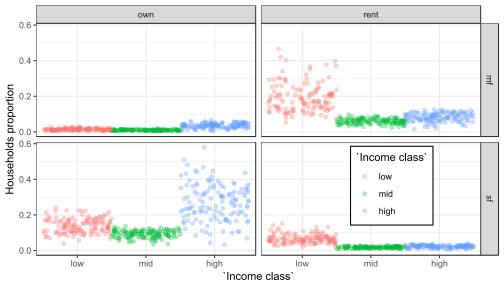
\includegraphics{Agenda_files/figure-latex/unnamed-chunk-3-1.svg}

\subsection{Residential solar potential (MWh/ household) in
Seattle}\label{residential-solar-potential-mwh-household-in-seattle}

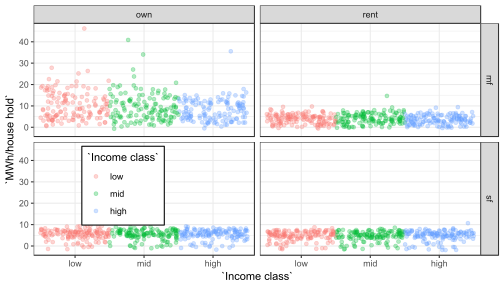
\includegraphics{Agenda_files/figure-latex/unnamed-chunk-4-1.svg}

\subsection{Histograms of multiple
variables}\label{histograms-of-multiple-variables}

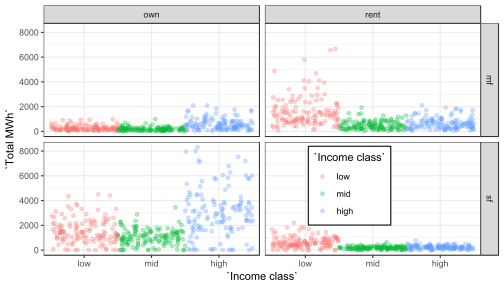
\includegraphics{Agenda_files/figure-latex/unnamed-chunk-5-1.pdf}

\subsection{Cor plot}\label{cor-plot}

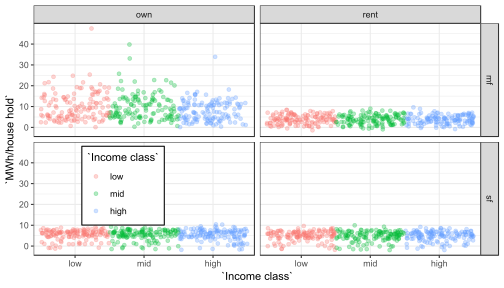
\includegraphics{Agenda_files/figure-latex/unnamed-chunk-6-1.pdf}

\subsection{Regression}\label{regression}

\begin{verbatim}
## 
## Call:
## lm(formula = sol_instl ~ hu_rnt + hu_med_val + black, data = fin[-c(1, 
##     2, 6, 7, 8, 9)])
## 
## Residuals:
##     Min      1Q  Median      3Q     Max 
## -8.0301 -1.7673 -0.4132  1.1725 14.2792 
## 
## Coefficients:
##               Estimate Std. Error t value Pr(>|t|)    
## (Intercept)  1.415e+01  1.770e+00   7.997 6.80e-13 ***
## hu_rnt      -1.901e+01  1.692e+00 -11.236  < 2e-16 ***
## hu_med_val   8.420e-06  1.953e-06   4.311 3.23e-05 ***
## black        7.972e+00  3.218e+00   2.477   0.0146 *  
## ---
## Signif. codes:  0 '***' 0.001 '**' 0.01 '*' 0.05 '.' 0.1 ' ' 1
## 
## Residual standard error: 2.859 on 127 degrees of freedom
## Multiple R-squared:  0.6207, Adjusted R-squared:  0.6117 
## F-statistic: 69.26 on 3 and 127 DF,  p-value: < 2.2e-16
\end{verbatim}

\subsection{Residual from the OLS}\label{residual-from-the-ols}

\begin{figure}
\centering
\includegraphics{./Figs/Residual.jpg}
\caption{Residual mapping}
\end{figure}

\subsection{Geographically weighted regression
(GWR)}\label{geographically-weighted-regression-gwr}

\begin{figure}
\centering
\includegraphics{./Figs/Residual-GWR.jpg}
\caption{Residual mapping for GWR}
\end{figure}

\subsection{Geographically weighted
impact}\label{geographically-weighted-impact}

\begin{figure}
\centering
\includegraphics{./Figs/Rental-w.jpg}
\caption{Rental proportion}
\end{figure}

\begin{figure}
\centering
\includegraphics{./Figs/H-value-w.jpg}
\caption{House median value}
\end{figure}

\begin{figure}
\centering
\includegraphics{./Figs/Black-w.jpg}
\caption{Black people proportion}
\end{figure}

\subsection{Factor analysis (Parallel
screen)}\label{factor-analysis-parallel-screen}

\includegraphics{Agenda_files/figure-latex/unnamed-chunk-8-1.pdf}

\begin{verbatim}
## Parallel analysis suggests that the number of factors =  4  and the number of components =  NA
\end{verbatim}

\subsection{Factor analysis (Plot)}\label{factor-analysis-plot}

\includegraphics{Agenda_files/figure-latex/unnamed-chunk-9-1.pdf}

\subsection{Factor analysis (Diagram)}\label{factor-analysis-diagram}

\includegraphics{Agenda_files/figure-latex/unnamed-chunk-10-1.pdf}

\subsection{Factor correlation for solar
installation}\label{factor-correlation-for-solar-installation}

\includegraphics{Agenda_files/figure-latex/unnamed-chunk-11-1.pdf}

\subsection{Factor regression}\label{factor-regression}

\begin{verbatim}
## 
## Call:
## lm(formula = fin[[16]] ~ dat[, 1] + dat[, 2] + dat[, 3])
## 
## Residuals:
##     Min      1Q  Median      3Q     Max 
## -6.2962 -2.0322 -0.5817  1.5500 17.9535 
## 
## Coefficients:
##             Estimate Std. Error t value Pr(>|t|)    
## (Intercept)   5.0904     0.2919  17.441  < 2e-16 ***
## dat[, 1]      2.2605     0.3361   6.726 5.34e-10 ***
## dat[, 2]     -1.1489     0.3472  -3.309  0.00122 ** 
## dat[, 3]     -0.9088     0.3001  -3.028  0.00298 ** 
## ---
## Signif. codes:  0 '***' 0.001 '**' 0.01 '*' 0.05 '.' 0.1 ' ' 1
## 
## Residual standard error: 3.34 on 127 degrees of freedom
## Multiple R-squared:  0.4823, Adjusted R-squared:   0.47 
## F-statistic: 39.44 on 3 and 127 DF,  p-value: < 2.2e-16
\end{verbatim}

\subsection{Kmeans}\label{kmeans}

\begin{verbatim}
##          ML2        ML3        ML1
## 1  0.8446908 -0.6505453 -0.4342311
## 2 -0.1748794  0.3173398  1.5743013
## 3 -0.7429633  0.4825947 -0.3462607
\end{verbatim}

\begin{verbatim}
## 
##  1  2  3 
## 52 26 53
\end{verbatim}

\includegraphics{Agenda_files/figure-latex/unnamed-chunk-13-1.pdf}

\subsection{Cluster within cluster sum of squares
(WCSS)}\label{cluster-within-cluster-sum-of-squares-wcss}

\begin{verbatim}
## [1] 251.739
\end{verbatim}

\includegraphics{Agenda_files/figure-latex/unnamed-chunk-14-1.pdf}

\subsection{Cluster plot}\label{cluster-plot}

\includegraphics{Agenda_files/figure-latex/unnamed-chunk-15-1.pdf}
\includegraphics{Agenda_files/figure-latex/unnamed-chunk-15-2.pdf}

\subsection{3D plot}\label{d-plot}

\begin{figure}
\centering
\includegraphics{./Figs/3D.jpg}
\caption{}
\end{figure}


\end{document}
